\section{Durchführung}
In diesem Versuch wird die in Abbildung~\ref{fig:aufbau}, die
[1] entnommen ist, schematisch dargestellte Apparatur
verwendet.  Dabei werden zwei Stäbe bei einseitiger und ein Stab bei
beidseitiger Auflage vermessen.  Bei der einseitigen Auflage wird ein
Stahlstab mit quadratischem Querschnitt und ein Aluminiumstab mit
kreisförmigem Querschnitt verwendet. Bei der beidseitigen Auflage wird
ein Messingstab mit quadratischem Querschnitt verwendet.

In der Abbildung ist bereits zu erkennen, wie die Durchbiegung eines
Stabes bei einseitiger Auflage vermessen wird. Es wird ein Gewicht am
freien Ende des Stabes aufgehängt, um dadurch ein maximales Drehmoment,
also eine maximale Durchbiegungs des Stabes zu erhalten. Nun fährt man
mit einer verschiebbaren Messuhr am Stab entlang und misst die
Durchbiegung in Abhängigkeit von der Entfernung zum Auflageort. In
diesem Versuch wird zu verschiedenen Entfernungen $x$ sowohl die
Durchbiegung $D_0(x)$ ohne Gewicht, als auch die Durchbiegung $D_M(x)$
mit Gewicht gemessen, sodass sich die tatsächliche Durchbiegung $D(x)$
nach Formel \eqref{eq:echte_durchbiegung} als Differenz der gemessenen
Werte ergibt.

Bei der beidseitigen Auflage wird das Gewicht an der Stabmitte
angebracht. Nun wird die Durchbiegung mit beiden verschiebbaren
Messuhren vermessen. Auch hier wird die Durchbiegung des unbelasteten
Stabes und die des belasteten Stabes gemssen, um die tatsächliche
Durchbiegung $D(x)$ nach Formel \eqref{eq:echte_durchbiegung} zu
erhalten.

\begin{equation}
\label{eq:echte_durchbiegung}
D(x) = D_n(x) - D_v(x)
\end{equation}

\begin{figure}
\centering
\includegraphics{aufbau}
\caption{Darstellung der verwendeten Apparatur. Die Abbildung ist aus
  \textcite{v103} entnommen.}
\label{fig:aufbau}
\end{figure} 
